{\small{
\begin{tabular}{c}
    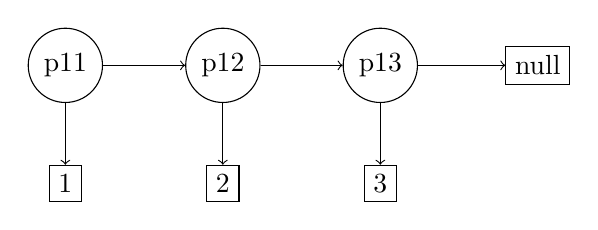
\begin{tikzpicture}
        \node[circle, draw] (n1) at (0,1.5) {p11};
        \node[circle, draw] (n2) at (2,1.5) {p12};
        \node[circle, draw] (n3) at (4,1.5) {p13};
        \node[draw] (null) at (6,1.5) {null};
        \node[draw] (v1) at (0,0) {1};
        \node[draw] (v2) at (2,0) {2};
        \node[draw] (v3) at (4,0) {3};
        \draw[->] (n1) --  node [above,midway] {\mynext} (n2);
        \draw[->] (n2) --  node [above,midway] {\mynext} (n3);
        \draw[->] (n3) --  node [above,midway] {\mynext} (null);
        \draw[->] (n1) --  node [midway] [above,midway,sloped] {\myvalue} (v1);
        \draw[->] (n2) --  node [midway] [above,midway,sloped] {\myvalue} (v2);
        \draw[->] (n3) --  node [midway] [above,midway,sloped] {\myvalue} (v3);
    \end{tikzpicture}
\\
\\
  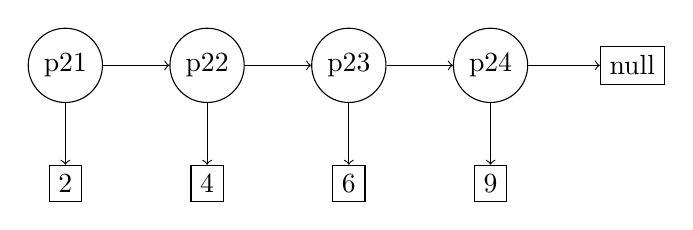
\begin{tikzpicture}
        \node[circle, draw] (n1) at (0,1.5) {p21};
        \node[circle, draw] (n2) at (1.8,1.5) {p22};
        \node[circle, draw] (n3) at (3.6,1.5) {p23};
        \node[circle, draw] (n4) at (5.4,1.5) {p24};
        \node[draw] (null) at (7.2,1.5) {null};
        \node[draw] (v1) at (0,0) {2};
        \node[draw] (v2) at (1.8,0) {4};
        \node[draw] (v3) at (3.6,0) {6};
        \node[draw] (v4) at (5.4,0) {9};
        \draw[->] (n1) --  node [above,midway] {\mynext} (n2);
        \draw[->] (n2) --  node [above,midway] {\mynext} (n3);
        \draw[->] (n3) --  node [above,midway] {\mynext} (n4);
        \draw[->] (n4) --  node [above,midway] {\mynext} (null);
        \draw[->] (n1) --  node [above,midway,sloped] {\myvalue} (v1);
        \draw[->] (n2) --  node [above,midway,sloped] {\myvalue} (v2);
        \draw[->] (n3) --  node [above,midway,sloped] {\myvalue} (v3);
        \draw[->] (n4) --  node [above,midway,sloped] {\myvalue} (v4);
    \end{tikzpicture}
\end{tabular}
}}
